All runs share the splits, corruption tensors, probe protocol, evaluation seeds, 15k steps, data order and parameter count
(1{,}412{,}864); only the mask sampler differs (Tab.~\ref{tab:h1}). The baseline was trained with 5 pretraining seeds, so
its seed standard deviation is known: 0.4 (clean), 0.8 (occ 25\%), 0.4 (occ 40\%), 1.0 ($\sigma{=}0.15$) points.

\begin{figure*}[t]
\centering
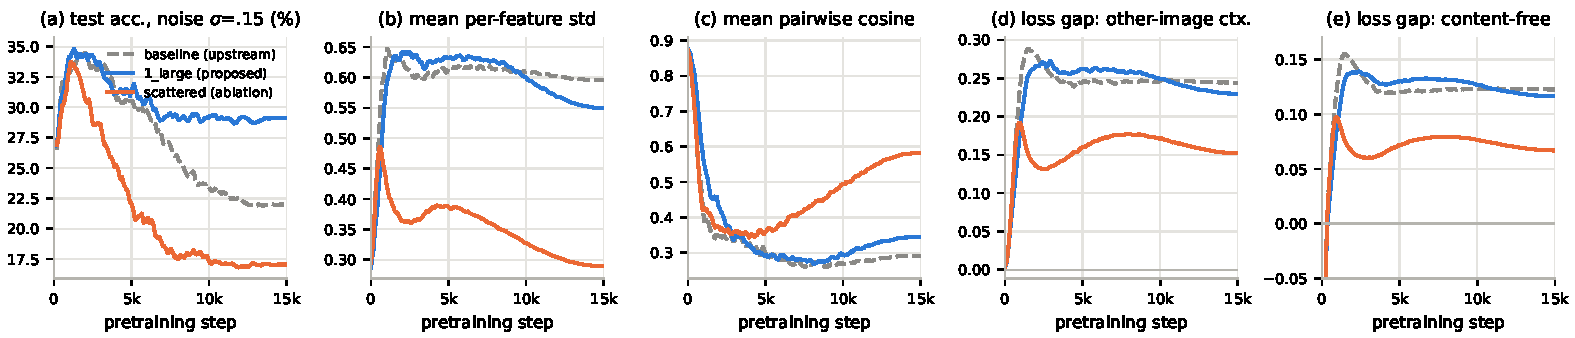
\includegraphics[width=\linewidth]{figures/fig_h1_mech.pdf}
\caption{Why one large target block is the most noise-robust geometry and scattered small blocks the least (seed 0, fixed
probe, 250-step moving average of the evaluations every 50 steps). (a) Test accuracy at noise $\sigma{=}0.15$. (b--c) Collapse
diagnostics of the pooled clean test features. (d) Held-out latent loss with another image's context minus the loss with the
image's own context: how much the prediction depends on the image's own content. (e) Loss of the content-free per-position
mean target minus the real-context loss: how much better than a position-only guess the predictor is.}
\label{fig:h1mech}
\end{figure*}

\textbf{Proposed: one large block (\texttt{1\_large}) -- the most noise-robust geometry.}
\obs Over 5 pretraining seeds 1\_large reaches \textbf{27.5$\pm$2.3} at $\sigma{=}0.15$, against 22.2$\pm$1.0 for the baseline
(+5.3 points, the largest gain of any masking geometry). 
% It keeps 55\% of its clean accuracy under $\sigma{=}0.15$
% (baseline 45\%, the other fixed-count samplers 42--46\%, scattered 34\%), and 
Its noise accuracy stops falling after
$\approx$6k steps while the baseline's keeps falling to the end (Fig.~\ref{fig:h1mech}a). Clean and occlusion accuracy
improve as well: 49.9$\pm$0.3 clean, 39.6$\pm$1.3 at 25\% and 31.7$\pm$0.5 at 40\% occlusion, i.e.\ +0.9, +2.3 and +2.8 points
over the baseline's 5-seed mean, each larger than both seed standard deviations. Its features keep the baseline's spread
(per-feature std 0.619 vs 0.618, pairwise cosine 0.29 vs 0.27, 5 seeds), and its prediction depends at least as much on
the image's own content: the loss rises by 0.267 when the context is taken from another image (baseline 0.252) and the
content-free target is 0.138 above the real-context loss (baseline 0.127; Fig.~\ref{fig:h1mech}b--e).
\interp With one contiguous hole of 35--42 patches the visible context is a ring around it, and most target tokens are
several patches away from any visible patch. The predictor can neither copy neighbouring texture nor fall back on the
target positions; it has to infer the hidden region from what the image shows as a whole (object, layout, colour). This
pushes the context encoder towards image-level, more semantic features, which i.i.d.\ pixel noise disturbs less than the
local detail it destroys. The same structure (``infer a large missing region from distant, peripheral context'') is what
the occlusion test asks. 
% The paper's principle that targets must be large enough to be semantic~\cite[Tab.~8]{assran2023ijepa}
% is about \emph{relative} scale: a CIFAR object fills most of a $32{\times}32$ frame, so the default $3{\times}3$-patch blocks
% ($12{\times}12$ px) are closer to object parts or texture, and a block covering half the image is closer to the object scale
% (\spec this would explain why larger-than-default targets help here but hurt on ImageNet, Tab.~8 of~\cite{assran2023ijepa}).
Two limits remain. Noise still moves the features as much as for the baseline (clean--noisy cosine 0.71 vs 0.71); what
improves is how much class information survives the shift. And 27.5\% is only at the level of a frozen random encoder
(26.6$\pm$1.3): the geometry slows the decline but does not make the encoder noise-invariant (that needs
Sec.~\ref{sec:noise}). On occlusion the contrast with the ablation is weaker than on noise: scattered (one seed) reaches
38.2/30.3 at 25/40\%, against 38.2/31.4 for 1\_large with the same seed, so H1's occlusion gain is only partly due to
contiguity. This is because in the ablation, we maintain that we should atleast get 20 context patches and 32 target patches 
after masking. So downstream occlusion performance does not vary much.

\textbf{Ablation: scattered small blocks -- local features, a position shortcut and the worst noise robustness.}
\obs Clean accuracy (50.1) and occlusion are unaffected, but $\sigma{=}0.05$ falls to 41.7 ($-$4.1) and $\sigma{=}0.15$ to
\textbf{17.0} ($-$5.2), the lowest of all runs (34\% of clean). The collapse diagnostics show why
(Fig.~\ref{fig:h1mech}b--c): from $\approx$1k steps on, the mean per-feature std stays at about half the baseline's
(0.290 vs 0.618 at 15k) and the mean pairwise cosine doubles (0.58 vs 0.29), while the effective rank stays high (62.6),
so this is not dimensional collapse. The content-ablated held-out losses (Fig.~\ref{fig:h1mech}d--e) are much closer to
the real-context loss: taking the context from another image raises the loss by only 0.152 (baseline 0.252, 1\_large 0.267),
and the content-free per-position mean target is only 0.067 above it (baseline 0.127, 1\_large 0.138).
\interp Every 2--6-patch target has visible context one patch away, so the predictor can solve the task from the target
\emph{positions} plus interpolation of neighbouring patches: the image's own content matters less (small other-image gap)
and a position-only guess is already close (small content-free gap). The context encoder is pushed towards local,
high-frequency patch detail with little image-level variation. Writing each pooled feature as a shared offset $m$ (the
mean over images) plus an image-specific deviation $v_i$, we measured $\lVert m\rVert{=}4.35$ (baseline) vs 3.91
(scattered) but an RMS deviation of 6.82 vs 3.33: the offset changes little and the image-specific part halves.
Per-feature std ignores $m$ and halves with $v$; the mean pairwise cosine is $\approx\lVert m\rVert^2/\mathbb E\lVert f\rVert^2$
(0.29 vs 0.58 measured), so it doubles. Because the probe standardises features, clean accuracy is unaffected, but pixel noise
destroys exactly the local detail these features encode and moves them far relative to the small differences between
images. 
% This matches the paper's finding that \texttt{random} patch targets give much less semantic features (17.6 vs
% 54.2,~\cite[Tab.~6]{assran2023ijepa}).

\textbf{Two large blocks.} Predicted as two separate sets of 16, \texttt{2\_large\_overlap} (two 16--30-patch blocks) is the
best single-seed run on clean (51.8, +2.9) and 10\% occlusion (48.9, +2.8) but not at 25/40\% occlusion (+0.5/$-$1.2) or
$\sigma{=}0.15$ (22.0). 
% (When both blocks were predicted as one 32-token set, i.e.\ as one large region, it had reached
% 40.0/30.9 at 25/40\% occlusion; \texttt{results/h1\_perblock}.) 
\texttt{2\_large\_nonoverlap} loses $-$3.2/$-$3.7 at 25/40\%
occlusion. 
% Two disjoint blocks of 16--20 patches that still leave 20 context patches fit on the $8{\times}8$ grid almost only as
% full-width or full-height bands (6.6 position draws per image and 0.13 block-size redraws per batch; Fig.~\ref{fig:masks}),
% so every target row or column borders a context band. \spec The task again becomes one-dimensional interpolation between
% neighbouring bands, and the model never has to infer a compact central region, which is what the occlusion test removes.

\textbf{Capped overlap between the 4 small blocks.} The overlap cap ($|A\cap B|/|A|<0.25$ for every pair) gains slightly
on clean (+1.4) but loses at 40\% occlusion ($-$1.5) and reaches only 21.5 at $\sigma{=}0.15$. 

\spec In the two large block experiments and the capped overlap experiment, although the experiments were run with only one 
seed, the downstream results do not differ much from the baseline results, since we maintain the context and token patch budgets
in all the experiments. These masking strategies still allow for context patches from the central region (the object region)
to be sampled during training, similar to the baseline masking strategy. Due to this we do not observe much differences in the 
results.

% Spreading the four small
% blocks apart does not change \emph{what} is predicted \emph{from what}: each block still has context next to it. The cap
% also lowers the context to 16.8 tokens (a 3$\times$4 batch almost always contains an image with only 16 available), with no
% measurable effect, so the context size in the 16--20 range is not limiting.

\textbf{Cost.} No sampler changes the parameter count (1{,}412{,}864). Training takes 516--566\,s per 15k steps on one L40S for the fixed-count samplers (baseline 581\,s)
and peak GPU memory is 0.26\,GB for them vs 0.33\,GB for the baseline, except for scattered, which makes
one predictor call per small block (6--16 per step): 852\,s and 0.51\,GB. Sampling costs 2--5\,ms per batch on the CPU.
